%13
\subsection{Elemek eltávolítása a veremből (pop)}
\begin{frame}
  \begin{columns}[c]
    \column{0.5\textwidth}
      \footnotesize
      \begin{exampleblock}{\textattachfile{verem2.cpp}{verem2.cpp}}
        \lstinputlisting[style=cpp,linerange={18-29},numbers=left,firstnumber=19]{verem2.cpp}
      \end{exampleblock}
    \column{0.45\textwidth}
      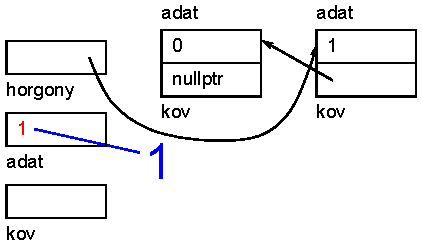
\includegraphics[width=\textwidth]{verem/verem10.pdf}
  \end{columns}
\end{frame}

%14
\begin{frame}
  \begin{columns}[c]
    \column{0.5\textwidth}
      \footnotesize
      \begin{exampleblock}{\textattachfile{verem2.cpp}{verem2.cpp}}
        \lstinputlisting[style=cpp,linerange={18-29},numbers=left,firstnumber=19]{verem2.cpp}
      \end{exampleblock}
    \column{0.45\textwidth}
      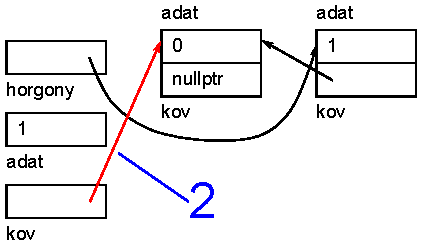
\includegraphics[width=\textwidth]{verem/verem11.pdf}
  \end{columns}
\end{frame}

%15
\begin{frame}
  \begin{columns}[c]
    \column{0.5\textwidth}
      \footnotesize
      \begin{exampleblock}{\textattachfile{verem2.cpp}{verem2.cpp}}
        \lstinputlisting[style=cpp,linerange={18-29},numbers=left,firstnumber=19]{verem2.cpp}
      \end{exampleblock}
    \column{0.45\textwidth}
      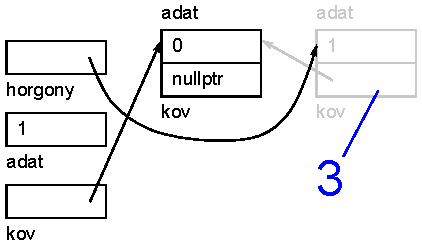
\includegraphics[width=\textwidth]{verem/verem12.pdf}
  \end{columns}
\end{frame}

%16
\begin{frame}
  \begin{columns}[c]
    \column{0.5\textwidth}
      \footnotesize
      \begin{exampleblock}{\textattachfile{verem2.cpp}{verem2.cpp}}
        \lstinputlisting[style=cpp,linerange={18-29},numbers=left,firstnumber=19]{verem2.cpp}
      \end{exampleblock}
    \column{0.45\textwidth}
      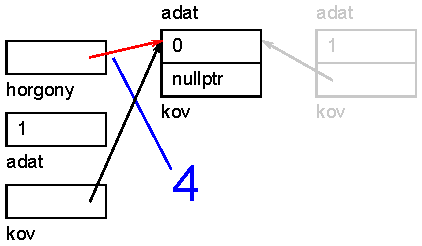
\includegraphics[width=\textwidth]{verem/verem13.pdf}
  \end{columns}
\end{frame}

%17
\begin{frame}
  \begin{columns}[c]
    \column{0.5\textwidth}
      \footnotesize
      \begin{exampleblock}{\textattachfile{verem2.cpp}{verem2.cpp}}
        \lstinputlisting[style=cpp,linerange={18-29},numbers=left,firstnumber=19]{verem2.cpp}
      \end{exampleblock}
    \column{0.45\textwidth}
      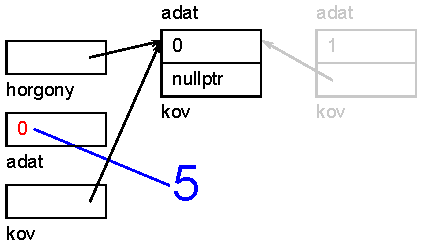
\includegraphics[width=\textwidth]{verem/verem14.pdf}
  \end{columns}
\end{frame}

%18
\begin{frame}
  \begin{columns}[c]
    \column{0.5\textwidth}
      \footnotesize
      \begin{exampleblock}{\textattachfile{verem2.cpp}{verem2.cpp}}
        \lstinputlisting[style=cpp,linerange={18-29},numbers=left,firstnumber=19]{verem2.cpp}
      \end{exampleblock}
    \column{0.45\textwidth}
      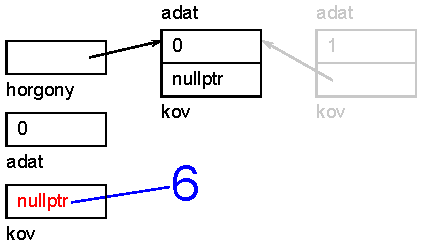
\includegraphics[width=\textwidth]{verem/verem15.pdf}
  \end{columns}
\end{frame}

%19
\begin{frame}
  \begin{columns}[c]
    \column{0.5\textwidth}
      \footnotesize
      \begin{exampleblock}{\textattachfile{verem2.cpp}{verem2.cpp}}
        \lstinputlisting[style=cpp,linerange={18-29},numbers=left,firstnumber=19]{verem2.cpp}
      \end{exampleblock}
    \column{0.45\textwidth}
      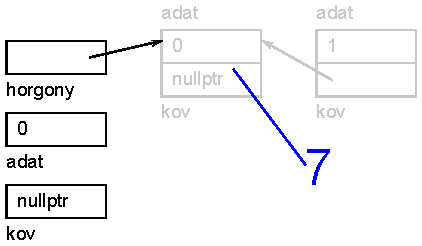
\includegraphics[width=\textwidth]{verem/verem16.pdf}
  \end{columns}
\end{frame}

%20
\begin{frame}
  \begin{columns}[c]
    \column{0.5\textwidth}
      \footnotesize
      \begin{exampleblock}{\textattachfile{verem2.cpp}{verem2.cpp}}
        \lstinputlisting[style=cpp,linerange={18-29},numbers=left,firstnumber=19]{verem2.cpp}
      \end{exampleblock}
    \column{0.45\textwidth}
      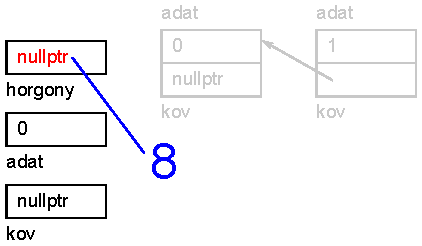
\includegraphics[width=\textwidth]{verem/verem17.pdf}
  \end{columns}
\end{frame}